\clearpage
% Introduction.tex
\chapter{Introduction}
\label{chap:introduction}

\section{Background}
\label{sec:background}
With a doubling of the world's elderly population, there is an urgent need for innovative and sustainable healthcare solutions to enable the eldest to live an independent, dignified, safe and responsible life. This is especially pressing in developing countries like Bangladesh where the majority of healthcare needs are unmet. Access to decent quality healthcare services is lacking and healthcare services are often geographically restrained; access to healthcare services is limited, specifically in rural or impoverished areas. Consequently, many elderly will be suffering from chronic illness or cognitive decline, or even social isolation without any regular basis of care as a result of the lack of health professionals, lack of awareness or high excessive costs to maintain ongoing treatment and supervision. 
Previous caregiving models are no longer sufficiently meeting elders' caregiving needs when the conditions of previous caregiving conditions (urbanization, migration working of younger family members and the economy) have changed so drastically. It is at this time that many elderly residents are left alone for long periods of time and lack conscious effort to take care of themselves. This condition exacerbates the rats of missing dose medications, experiencing health concerns with no supervision and their mental health deteriorating. Caregivers, whose duties might also include child care (elementary or older children in education, personal care, etc.) or professional employment, experience progressive feelings of burnout for their responsibilities, but also because of limited family involvement, assistance and limited to non-existent resources.
This is of great importance when considering that the majority of individuals will be acquiring these devices as their sole means of pursuing quality daily living assistance. In addition, we encourage users to address the design of the functionalities they wish to use in Medora. 

With Medora we aim to transform the traditional care role of a caregiver to a more dynamic living companion to an elderly individual. Medora is able to assist with prompting, monitoring and social interaction/engagement to provide an individualized experience for daily living assistance. As pointed out earlier, most products need for an individual to have emergent technological skills or even moderate use of new technology and if Medora can simplify this process, we feel that we will have added considerable value. In conclusion, we have developed a care robot that can assist with monitoring, prompting, social interaction and engagement. Medora's objective is to enable the elderly individual, with social engagement onboard, the ability to increasingly retain their independence and live more comfortably at home.

\begin{figure}[h]
    \centering
    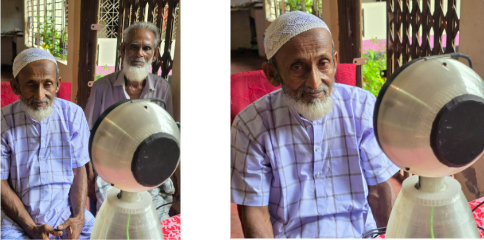
\includegraphics[width=0.7\textwidth]{Medora_thesis (1)/pics/thesis/eiwm.png}
    \caption{Medora interacting with Elderly
}
    \label{fig:Medora interacting with Elderly}
\end{figure}

Instead of a high-end robot solution centered around one task, or expensive hardware requiring proprietary software and hardware, Medora is a concept for scalability and local empowerment effort for technology. There are many ways you can scale the Medora from different perspectives, including local upgrades, expansions like health data logging, voice commands in local languages, and remote monitoring.  This is not only a technology solution, but also a community based innovation model to encourage local participation in healthcare tech development. 
In a country like Bangladesh, where the rural health care infrastructure is lagging behind and supporting an elderly member of the family is typically a role assumed by an untrained family member, Medora can serve a role in between the patient and the health care systems. Marketed as a low power consumer with no wires or computer connectivity, and being able to work in a local network or some level without being hardwired to an internet or sense access to electrical power, with someone who is caring for an elderly family member, Medora could provide an invaluable tool/resource in a rural community and build a pathway toward better health.
 Medora is a robot that it’s a companion, a reminder system, a health assistant designed to tackle the challenges faced when providing elderly care in the real world. Medora is a step forward for inclusive, affordable, and intelligent health care support for communities who need it the most. By relieving the burden on caregivers, by facilitating an easy intake of medication, by enhancing everyday living for the elderly, Medora contributes to the wider goal of healthcare for everyone, and provides an example of how local inspiration can produce global innovation.



\section{Problem Statement}
\label{sec:Problem Statement}
With the growing statistic of the older adult population worldwide, many are still experiencing barriers connected sense of freedom, medical illnesses, reduced friendship networks, lack of confidence, and  loneliness. Aging-related loss of physical and mental functions are combined with chronically diseases and lower socialisation may profoundly affect the quality of life of older individuals. Situations can be worse in developing regions, where Cleanup challenges These problems can be worse in developing countries, where health care systems are often underresourced and face a shortage of professional caregivers or modern technologies.

While there are many assistive technologies that have been designed to address issues related to elder care, these solutions are for the most part fragmented and do not allow for integration across the multiple and complex needs of older adults. For example, certain options focus solely on health monitoring via wearables that monitor a person's health condition through devices that track vitals and other information. Others focus on social interaction with the use of companion robots. Very few systems would combine physical and emotional support, and functional aspects into one cohesive platform.

Common limitations in current solutions include:

\begin{itemize}[noitemsep]
    \item High costs and proprietary designs that prevent easy access;
    \item Lack of interoperability between health monitoring and interactive components;
    \item Limited individual user personalization or adaptability;
    \item Impersonal interactions that are appear robotic and mechanical.
\end{itemize}

Most importantly, few robotic systems provide compelling, human-like engagement and provide basic healthcare support, like real-time temperature monitoring and medication reminders- which provide daily care for the elderly but are usually provided by separate systems or added manually when needed. 
This research project addresses the above gaps and develops Medora, a low-cost multifunctional medical aide robot. Medora is not a typical assistive technology. Medora unique integrates:

\begin{itemize}[noitemsep]
    \item Natural voice-based interaction with personalized and intuitive communication;
    \item Facial and emotion recognition to understand the user's mood and offer appropriate replies;
    \item Medication reminders for treatment compliance;
    \item Real-time temperature monitoring for fundamental healthcare data, through one platform.
\end{itemize}

Most importantly, Medora combines all the above abilities in one user-friendly system, which unifies healthcare functionality while providing affective presence- an area not addressed by existing robotic technologies. Built on low-cost, readily available, open cooperative platforms,Medora offers a scalable solution for families and care-givers.



\section{Objectives}
\label{sec:Objective}


The primary objective of this project is to develop Medora, an affordable, emotion-aware assistive robot designed to support elderly individuals in their daily lives. Unlike conventional assistive technologies, Medora integrates facial recognition, emotion detection, natural voice interaction, health monitoring, and medication management into a single, user-friendly system. Built on a Raspberry Pi 4B and leveraging open-source frameworks such as OpenCV, DeepFace, and Google Text-to-Speech, the robot delivers personalized care while remaining cost-effective and scalable.

Medora’s goals include:

Enhancing elderly independence through natural, voice-based interaction that eliminates the need for complex manual controls.

Providing health monitoring by integrating sensors such as the DS18B20 for real-time temperature tracking.

Improving medication adherence with scheduled reminders, verbal prompts.

Offering emotional support by recognizing user emotions and adapting responses to promote companionship and well-being.

Reducing caregiver burden through automated monitoring, reminders.

Ultimately, the objective is to create a human-centered, intelligent, and accessible elderly care solution that enhances quality of life, fosters emotional connection, and extends healthcare access, particularly in resource-limited or rural environments.

\section{Scope of the Study}
\label{sec:Scope of the Study}

This research is concerned with the design and development of a multi-functional medical assistive robot system for elderly users. The intention is to use the robot in indoor and regulated environments (e.g., homes, care homes) to evaluate the efficiency of the robot assisting elderly users in their activities of daily living and health monitoring. The main functions of the robot are the following:

\begin{itemize}
    \item \textbf{Voice Interaction:} The robot will have a voice interface based on Natural Language Processing (NLP) to facilitate easy and intuitive communication between the user and the system.
    
    \item \textbf{Face and Emotion Recognition:} AI-based face recognition and emotion recognition will allow the robot to recognize users and understand their emotional context, which will allow the robot to respond adaptively and personalized to each user.
    
    \item \textbf{Medication Reminder:} The robot will have a voice interface based on Natural Language Processing (NLP) to facilitate easy and intuitive communication between the user and the system.
    
    \item \textbf{Real-time Body Temperature Monitoring:}  Real-time body temperature monitoring: The robot is required to have sensors to monitor vitals signs but the focus will be real-time body temperature.
\end{itemize}

The study focuses on the design and implementation of the robot for formally controlled indoor spaces. This study does not consider large-scale clinical trails or configurations for outdoor uses. The robot is designed to assist caregivers, not replace human interactions completely. The main goal is to create a representationally designed, affordable and accessible elderly care solution improving quality of life while reducing caregiver burden.





\section{Research Questions}
\label{sec:Research Question}

This research addresses the following questions:

\begin{enumerate}
    \item How can a multifunctional medical assistive robot be effectively designed and implemented using Raspberry Pi and IoT technologies for elderly care?
    
    \item What methods can improve the accuracy and reliability of facial recognition and emotion detection to enable personalized interaction?
    
    \item How can real-time health monitoring, including body temperature measurement, be integrated into the robot to support elderly users’ well-being?
    
    \item How effective is the interactive medicine reminder system in improving medication adherence among elderly users?
    
    \item How can voice-based interaction be optimized to provide intuitive and user-friendly communication between the robot and elderly users?
\end{enumerate}

This study aims to answer the research questions and create an effective and user-friendly solution for elderly care that can improve the quality of life for elderly people, while also relieving some burden on caregivers. As the robot incorporates AI and IoT technologies, it has new capabilities for remote health monitoring and telemedicine, which can be very beneficial for elderly people in rural or underserved communities.






\section{Thesis Structure}

This thesis is organized into seven chapters, each addressing a specific aspect of the project. The structure is designed to provide a logical progression from the introduction and background to implementation, results, and conclusions. The chapters are outlined as follows:

\begin{itemize}
    \item \textbf{Chapter 1: Introduction} \\
    This chapter provides an overview of the background, problem statement, research objectives, scope, research questions, conceptual framework, and thesis structure.
    
    \item \textbf{Chapter 2: Literature Review} \\
    This chapter reviews existing research and technologies related to medical assistive robots, AI technologies, Raspberry Pi applications, and IoT in elderly care.
    
    \item \textbf{Chapter 3: System Design} \\
    This chapter describes the hardware components, software design, framework and the methodology of the robot.
    
    \item \textbf{Chapter 4: System Design and Implementation} \\
    This chapter provides detailed explanations of the robot's design, components assembly, and the software implementation.
    
    \item \textbf{Chapter 5: Data Survey} \\
    This chapter presents the survey data collected, interview process , analysis, and insights relevant to the research.
    
    \item \textbf{Chapter 6: Results and Discussion} \\
    This chapter analyzes the robot's performance, presenting findings, evaluating outcomes, and addressing limitations.
    
    \item \textbf{Chapter 7: Conclusion and Future Work} \\
    This chapter summarizes the key findings and contributions of the research and offers recommendations for future studies.
\end{itemize}
